\begin{figure}[t]
	\newcommand{\minipagesize}{0.5}
	\centering
    \begin{minipage}{\minipagesize\linewidth}
        \centering
        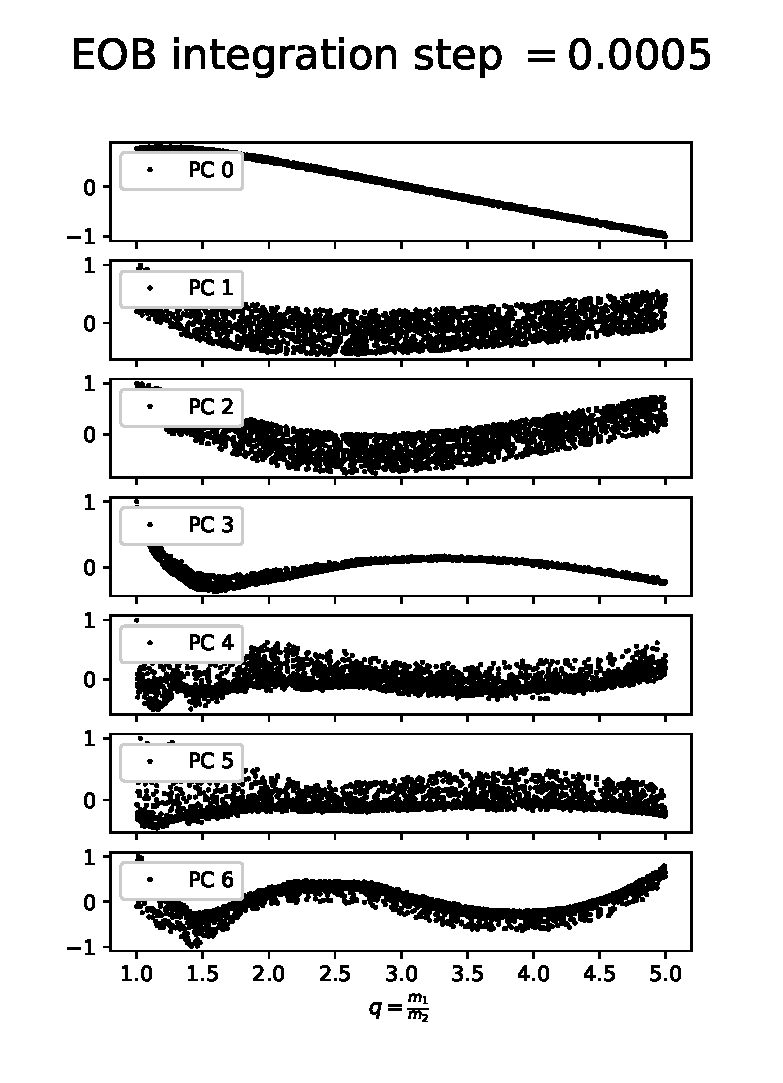
\includegraphics[width=\linewidth]{PC_q_noise3}
    \end{minipage}\hfill
    \begin{minipage}{\minipagesize\linewidth}
        \centering
        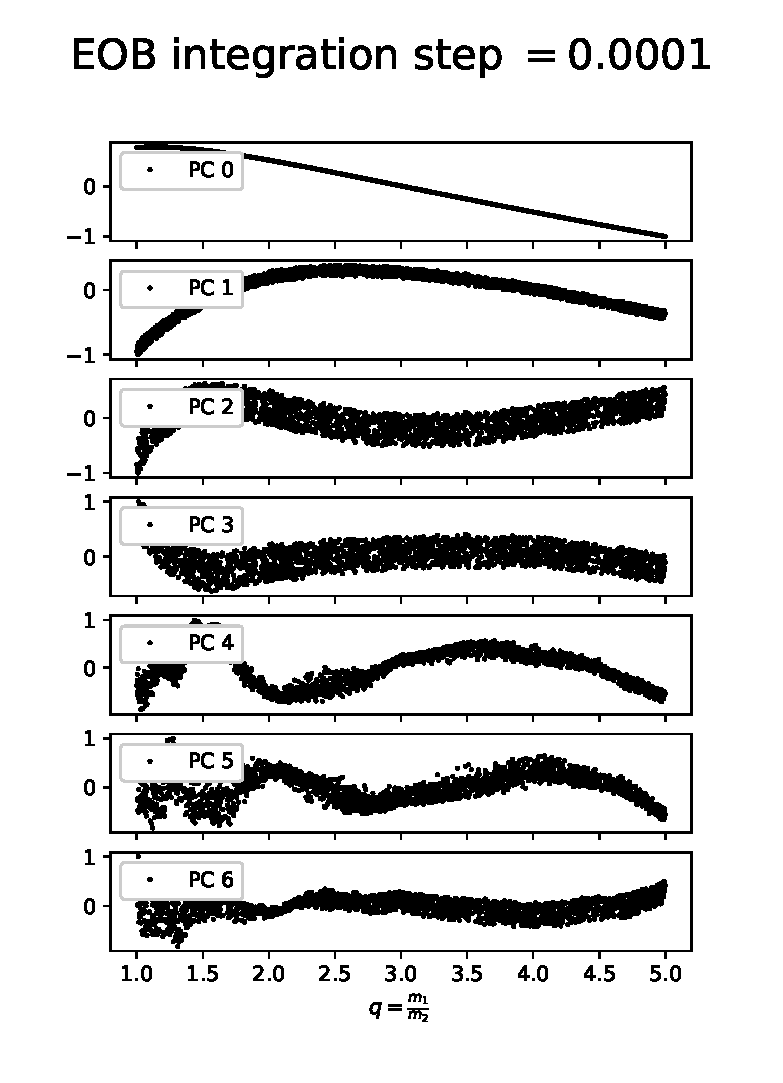
\includegraphics[width=\linewidth]{PC_q_noise2}
    \end{minipage}\vfill
    \begin{minipage}{\minipagesize\linewidth}
        \centering
        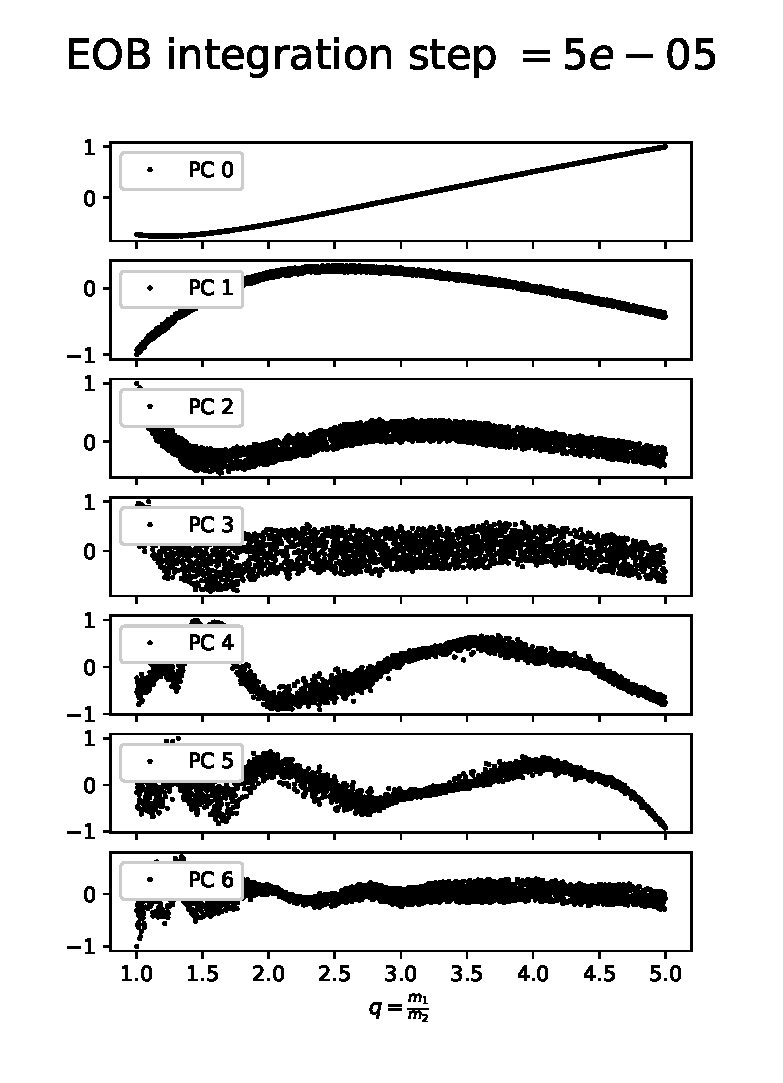
\includegraphics[width=\linewidth]{PC_q_noise1}
    \end{minipage}\hfill
    \begin{minipage}{\minipagesize\linewidth}
        \centering
        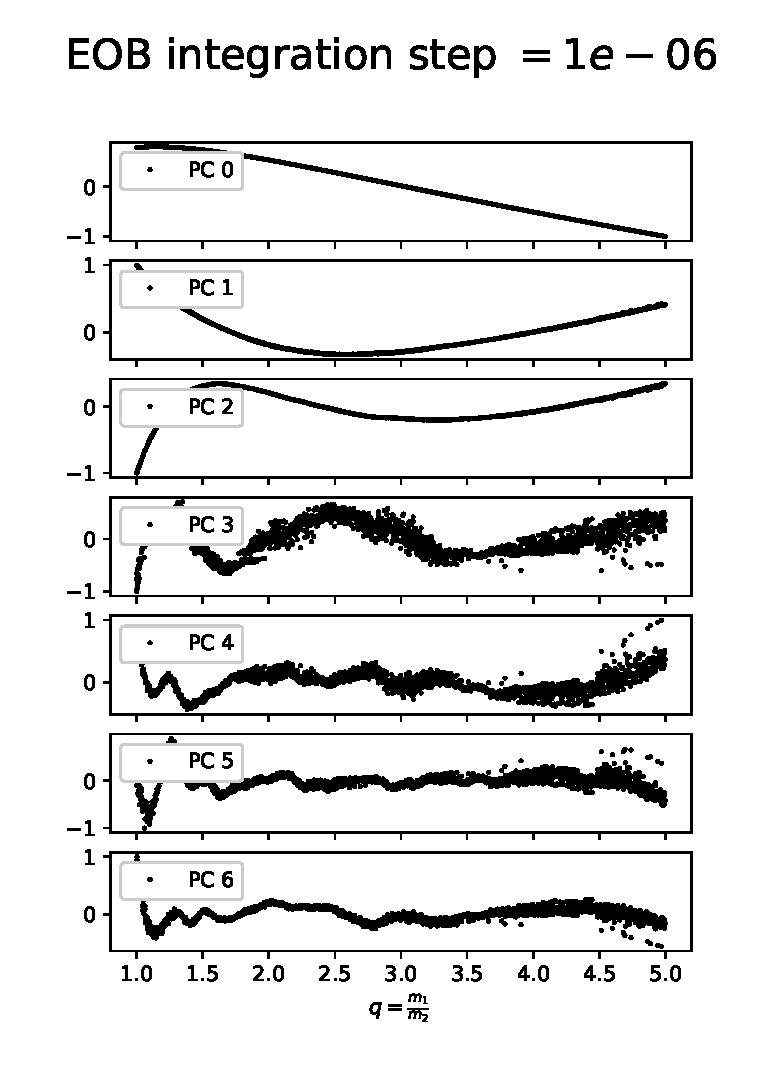
\includegraphics[width=\linewidth]{PC_q_noise0}
    \end{minipage}
	\caption{We represent here the projection of a waveform on the first 6 PCs as a function of the mass ratio $q$. Each point represents the projection coefficient on the PC shown in the label. Every waves is generated with $s_1 = -0.3$ and $s_2 = 0.2$.
Each columns display a dataset with a different EOB integration time step (the other hyperparameters being fixed).
}
	\label{fig:PC_q_noise}
\end{figure}

\section{Some issues on EOB accuracy}
We report below some remarks on the accuracy of EOB surrogate models. The discussion refers to model \texttt{SEOBNRv2}, but it is valid to other models of the same family.
\par
PCA provides a perturbative expansion of each datapoint in a dataset; as the perturbative order increase, the reconstruction error decreases. For this reason, PCA is able to explain the data up to a very small scale of observation.
As the dimensional reduction is pushed to higher PCs, numerical errors, due to a finite integration step $t_{step}$, enters the PCA resolution. This is inevitable as some amount of numerical noise cannot be avoid.
This is clearly visible in figure~\ref{fig:PC_q_noise}, where we reported the values of projection of several WFs on the first 6 PCs, plotted against the mass ratio $q$ (for fixed values of spins): this is the objective of the regression performed by the MoE. In each panel, we vary the magnitude of $t_{step}$.
\par
As the dimensional reduction is pushed to higher PCs, numerical errors, due to a finite $t_{step}$ makes up a noisy relation.
The effect of a decrease of $t_{step}$ is to lower the order at which the numerical noise enters.
When too much numerical noise arises (as is the case for higher PC in PCA perturbative expansion), the regression is uneffective. 
For this reason it is important to have numerical noise under control. If it is too high, the fit will stop at lower PCs and the regression will generalize the data poorly.
\par




